\providecommand{\main}{../../../..}
\documentclass[\main/dresen_thesis.tex]{subfiles}

\begin{document}
  \label{sec:looselyPackedNS:nanoparticle:xrd}
  \begin{figure}[tb]
    \centering
    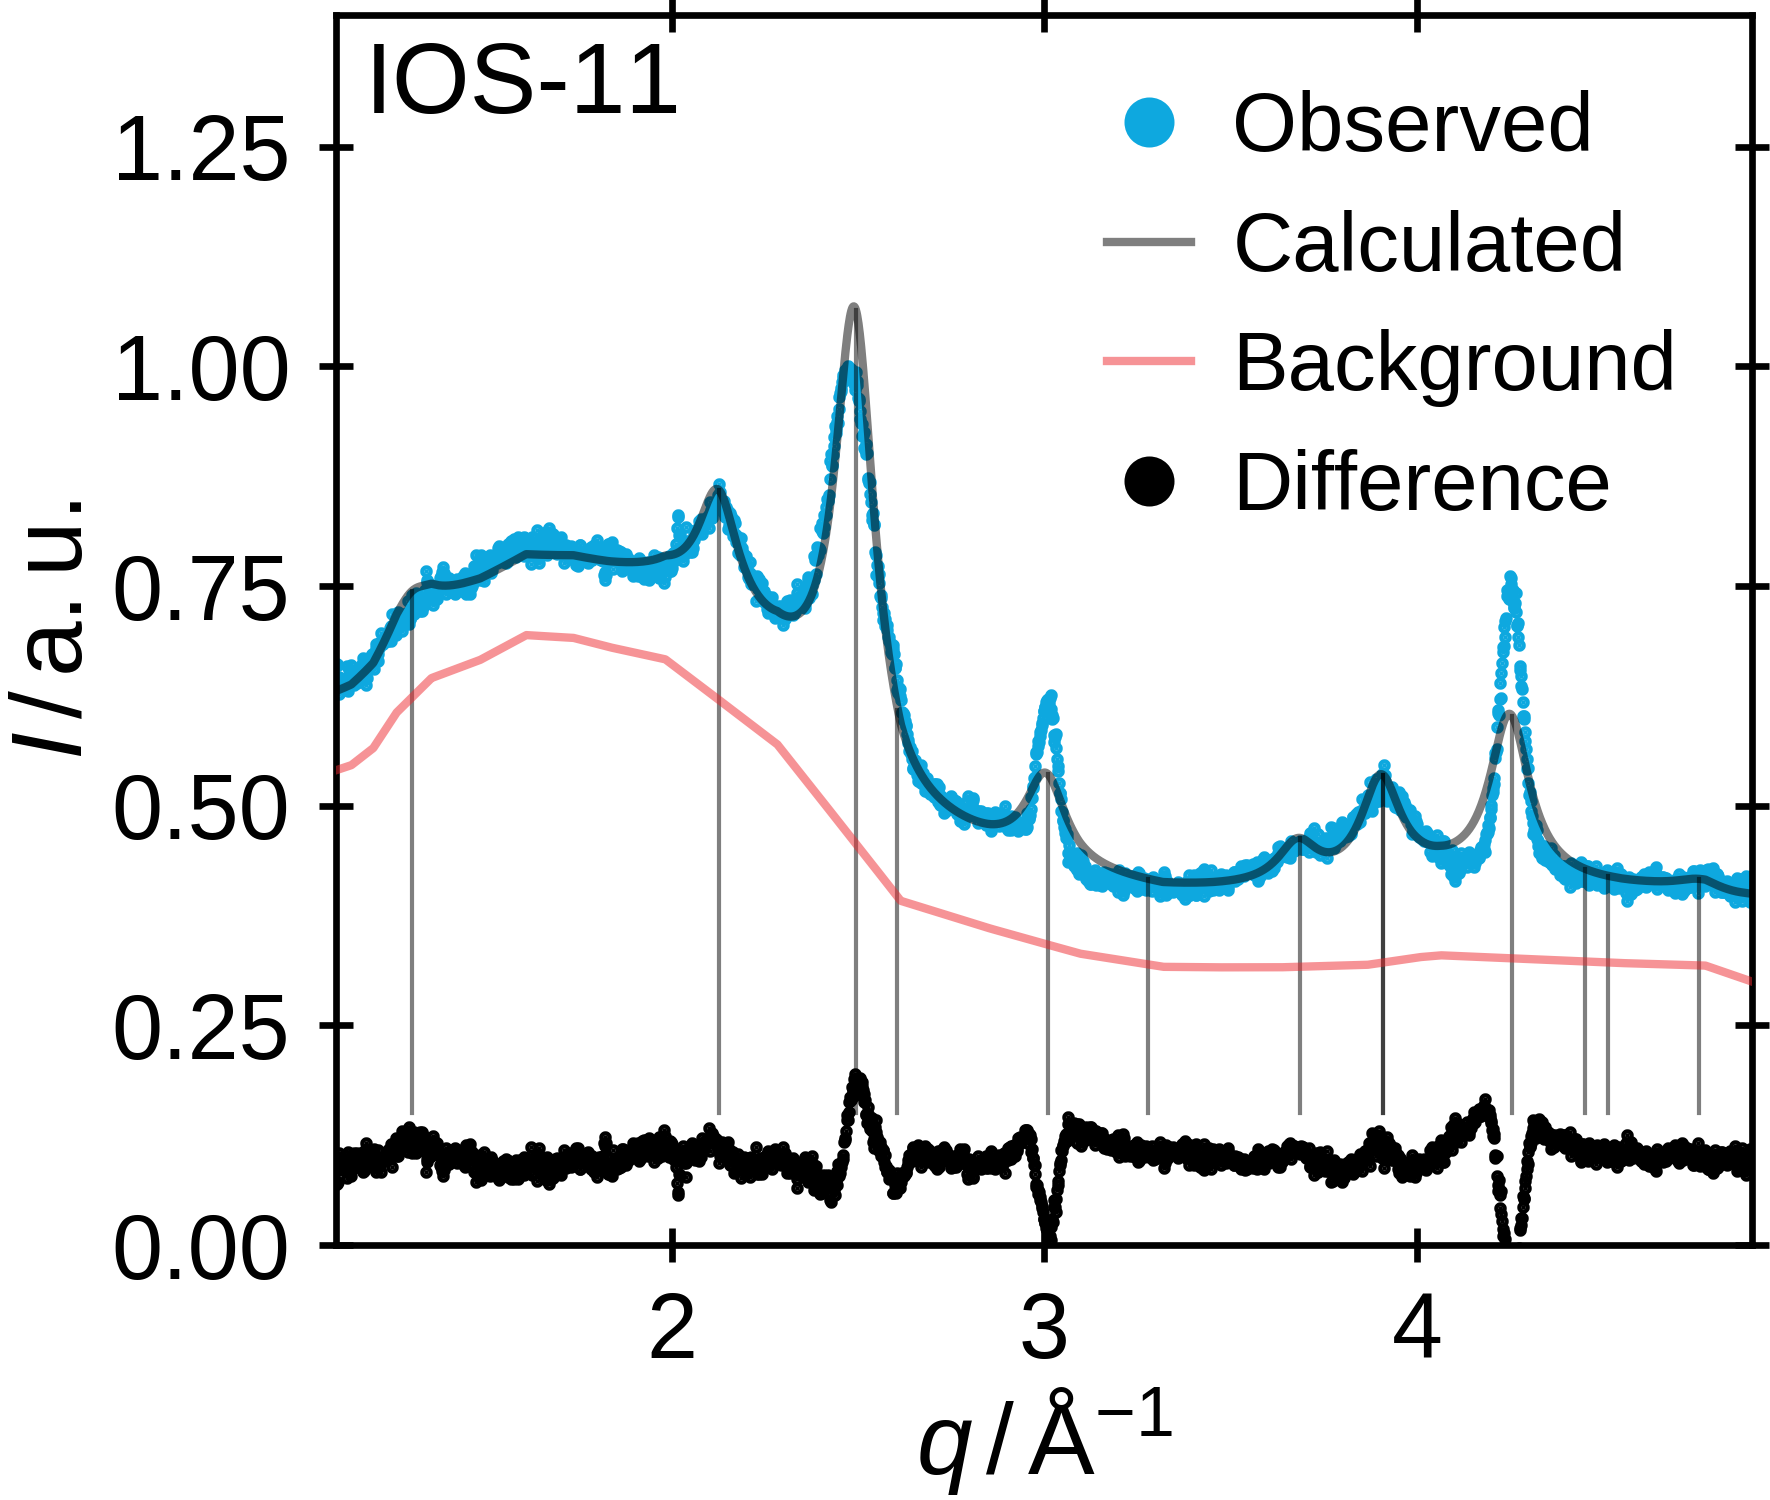
\includegraphics{looselyPackedNP_XRD_Fe2O3IOS-11}
    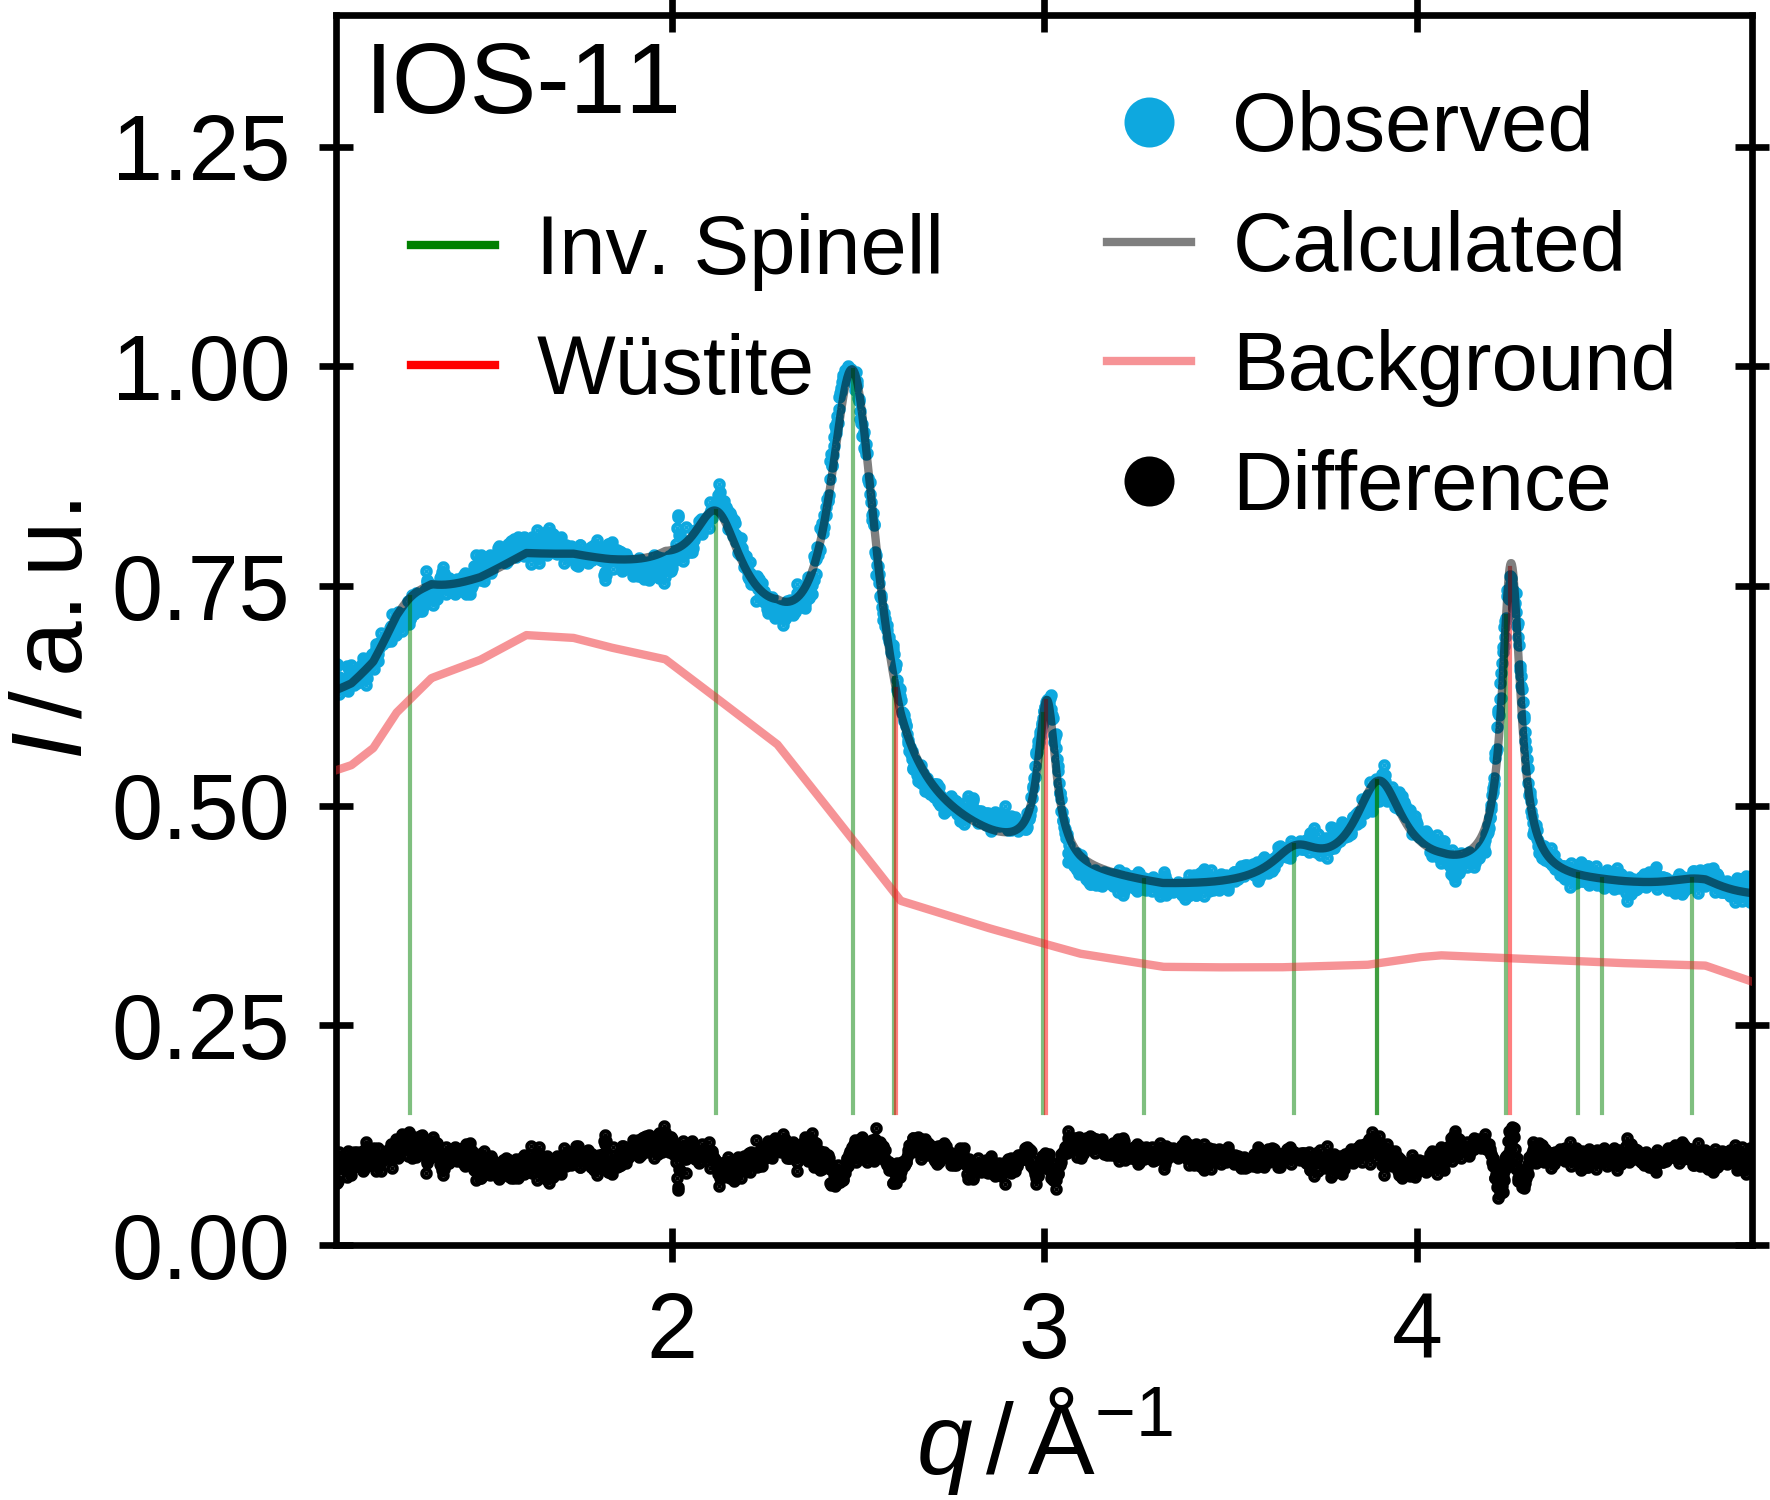
\includegraphics{looselyPackedNP_XRD_Fe2O3WustiteFit_IOS-11}
    \caption{\label{fig:monolayers:nanoparticle:xrd}XRD of IOS-11, once with a LeBail fit of a inverse spinell phase (left) and once with a LeBail fit where a sum of an inverse spinell and a w\"ustite phase is assumed. The manually estimated background is shown as red line.}
  \end{figure}

  In \reffig{fig:monolayers:nanoparticle:xrd} the diffraction data of IOS-11, and two performed LeBail fits are shown, to determine the phase, the lattice constant and the average crystallite size of the particles.
  On the left a LeBail fit is refined, where only an inverse spinell phase as expected from maghemite or magnetite.
  And on the right LeBail fit, both an inverse spinell and w\"ustite phase is refined.
  For both approaches the parameters of the refinement, the lattice constants $a$ and the Lorentzian isotropic size parameter $Y$ are summarized in \reftab{tab:looselyPackedNS:nanoparticle:discussion:xrdLeBail}.

  It is clearly visible in the LeBail fit of only a single phase that the LeBail fit does not properly describe the measured XRD data.
  The reflections around $3 \unit{\angstrom}$ and $4.2 \unit{\angstrom}$ are badly described, as the data shows a sharper peak width in these cases.
  By adding the w\"ustite phase, these problems are alleviated and the whole range is well described.

  \begin{table}[ht]
    \centering
    \caption{\label{tab:looselyPackedNS:nanoparticle:discussion:xrdLeBail}LeBail refinement parameters for the two fits to IOS-11 shown in \reffig{fig:monolayers:nanoparticle:xrd}. Given are the parameters of the lattice constants $a$ and the Lorentzian isotropic size parameter $Y$ for each phase. Additionally, the calculated crystallite size $L$ from the Debye-Scherrer equation is given for each phase, as well as the wavelength $\lambda$ used at each measurement, the figure of merit $\chi^2$ and the agreement factors $R$.}
    \begin{tabular}{ l | l | l }
      \hline
      \rule{0pt}{2ex} & \multicolumn{2}{c}{\textbf{IOS-11}}\\
      \hline
      \hline
      \rule{0pt}{2ex}space group & $Fd\bar{3}m$ (No. 227) & + $Fm\bar{3}m$ (No. 225)\\
      \hline
      \rule{0pt}{2ex} $a_\mathrm{inv. spinell} \,/ \unit{\angstrom}$         & $8.3729(4)$ & $8.3843(3)$  \\
      \rule{0pt}{2ex} $Y_\mathrm{inv. spinell} \,/ \unit{^\circ}$            & $1.778(8)$  & $2.198(5)$   \\
      \rule{0pt}{2ex} $a_\textsf{w\"ustite}     \,/ \unit{\angstrom}$        &             & $4.1819(1)$  \\
      \rule{0pt}{2ex} $Y_\textsf{w\"ustite}     \,/ \unit{^\circ}$           &             & $0.755(3)$   \\
      \hline
      \rule{0pt}{2ex} $L_\mathrm{inv. spinell} \,/ \unit{nm}$                & $3.161(1)$  & $2.557(1)$ \\
      \rule{0pt}{2ex} $L_\textsf{w\"ustite}      \,/ \unit{nm}$              &             & $7.442(2)$ \\
      \hline
      \rule{0pt}{2ex} $\lambda \,/ \unit{\angstrom}$                         & \multicolumn{2}{c}{$1.54056$}\\
      \hline
      \rule{0pt}{2ex} $\chi^2$                                               & $7.00$      & $1.70$ \\
      \rule{0pt}{2ex} $R_p$                                                  & $2.52$      & $1.52$ \\
      \rule{0pt}{2ex} $R_{wp}$                                               & $3.93$      & $1.94$ \\
      \rule{0pt}{2ex} $R_{exp}$                                              & $1.49$      & $1.48$ \\
      \rule{0pt}{2ex} $R_{f, \, \mathrm{inv. spinell}}$                      & $0.15$      & $0.10$ \\
      \rule{0pt}{2ex} $R_{f, \, \text{w\"ustite}}$                           &             & $0.15$ \\
      \hline
    \end{tabular}
  \end{table}

  \paragraphNewLine{Lattice constant}
    The nanoparticle IOS-11 shows two phases, an inverse spinell phase with a lattice constant of $8.3843(3) \unit{\angstrom}$ and a w\"ustite phase with a lattice constant of $4.1819(1) \unit{\angstrom}$.
    These values can be compared to the bulk values of the lattice constant of magnetite/maghemite ($a_\mathrm{magnetite} \eq 8.396 \unit{\angstrom}$, $a_\mathrm{maghemite} \eq 8.340 \unit{\angstrom}$) \cite{Cornell_2003_Their} and to the bulk value of w\"ustite ($a_\mathrm{FeO} \eq 4.33 \unit{\angstrom}$ \cite{Hentschel_1970_Stoich}).

    The observed lattice constant for the inverse spinell phase lies in between the bulk values of magnetite and maghemite, and the lattice constant of the w\"ustite phase is below that of the bulk literature value.
    Both observations are also made in literature \cite{Wetterskog_2013_Anoma}.
    The reduced lattice constant for the w\"ustite core is explained by the lattice mismatch with respect to the inverse spinell shell and thereby a strong pressure that is exerted on the core that results in a compression.
    The lattice constant of the shell shows the trend to decrease from the magnetite literature value towards the maghemite value with increasing oxidation time.
    From the here measured lattice constant, the assumptions can be made that the shell is close to a magnetite phase \cite{Cervellino_2014_Latti}.
    As the precision of determining the oxidation state from the lattice parameter is however large, especially for small sized crystallite sizes, it has to be kept in mind that this assumption introduces a potential systematic error.

  \paragraphNewLine{Crystallite Size}
    From the Lorentzian isotropic size parameters, the crystallite sizes are determined to $7.442(2) \unit{nm}$ for the w\"ustite core and $2.557(1) \unit{nm}$ for the inverse spinell phase.
    The obtained sizes from XRD are comparable to the total particle size observed in TEM ($10.95(5) \unit{nm}$).
    The sum of the core and two times the shell thickness ($12.556(2)$) is slightly larger than the size from TEM.
    This is however conceivable from the core-shell structure if the scattering from both sides of the shell is partially coherent and therefore the sizes do not add up linearly.

  % \paragraphNewLine{Density}
  %   Due to the partial oxidation of the shell and the complex core-shell structure, the density can only be roughly estimated.

  %   To avoid introducing systematic errors by assuming a wrong phase of the shell, the density can be given by 5.2(1) g/mL
\end{document}